\chapter{Analysis}

\section{Requirements}

In this section, we outline the functional and non-functional requirements necessary for the successful implementation of the project.

\subsection{Functional Requirements}

\subsubsection{For Administrators:}

\begin{itemize}
    \item Administrators must be able to log in to the application.
    \item Administrators must be able to log out of the application securely.
    \item Administrators must be able to create new configurations for experiments.
    \item Administrators must be able to create experiments based on the configurations they have defined.
    \item Administrators must be able to initiate experiments and oversee their execution.
    \item Administrators must possess the authority to perform CRUD operations on configurations and experiments.
\end{itemize}

\subsubsection{For Users:}

\begin{itemize}
    \item Users must be able to log in to the application.
    \item Users must be able to log out of the application securely.
    \item Users must be able to register for a new account within the application.
    \item Users must be able to monitor real-time progress of experiments.
    \item Users must be able to search for experiments based on configuration and experiment names.
\end{itemize}

\subsection{Non-Functional Requirements}

\begin{enumerate}
    \item \textbf{Performance:} The system must handle a large number of concurrent users without significant performance degradation. Response times for critical operations should be kept within acceptable limits.
    \item \textbf{Reliability:} The system should be highly available with minimal downtime. Data integrity must be maintained at all times.
    \item \textbf{Security:} User authentication and authorization mechanisms must be implemented. Data transmission must be encrypted.
    \item \textbf{Scalability:} The system should scale horizontally to accommodate increasing user loads and data volumes.
    \item \textbf{Usability:} The user interface must be intuitive and error messages must be informative.
    \item \textbf{Maintainability:} The codebase must be well-organized and documentation must be comprehensive.
    \item \textbf{Compatibility:} The application must be compatible with a wide range of web browsers and devices. Integration with external systems must be seamless.
\end{enumerate}

\subsection{Constraints/Other Requirements}

\begin{itemize}
    \item \textbf{Regulatory Compliance:} The application must comply with relevant laws and regulations.
    \item \textbf{Hardware Requirements:} Specific hardware specifications may be necessary for hosting.
    \item \textbf{Localization Requirements:} The application may need to support multiple languages.
    \item \textbf{Data Migration:} Data from existing systems may need to be migrated.
    \item \textbf{Interact with FL Director:} Integration with the FL Director, including defining message formats and communication technologies.
    \item \textbf{Data Variability and Schemaless Handling:} The application must be capable of handling variable and schemaless data.
    \item \textbf{Deployment on Three Different Nodes:} The application must be deployed on separate nodes for redundancy and reliability.
\end{itemize}

\newpage
\section{Use Case Diagram}
\subsection{Actors}

The actors who can interact with the web console system consist of the following:
\begin{itemize}
    \item \textbf{User:} The user is the actor who can browse the system to view running and completed experiments and their results.
    \item \textbf{Admin:} The admin is the actor who can manage the system, including creating and deleting configurations and experiments, and viewing the results of experiments.
\end{itemize}

\begin{figure}[ht!]
    \centering
    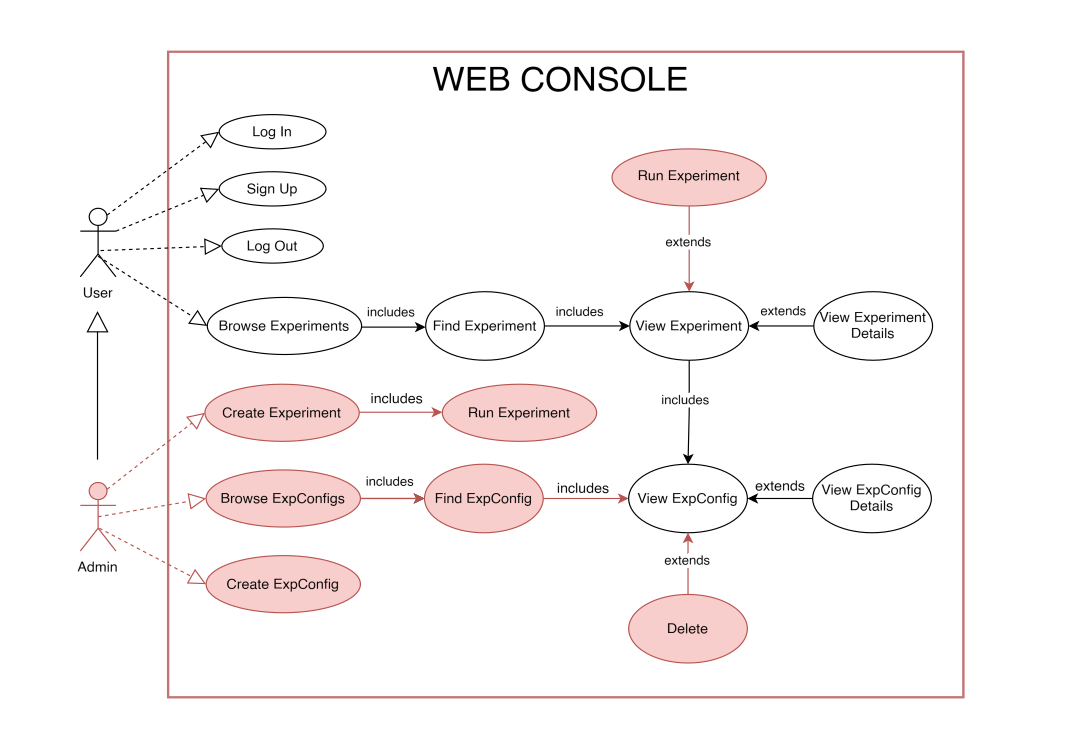
\includegraphics[width=\textwidth]{images/2_analisys/FL_use_case.png}
    \caption{Use Case Diagram}
    \label{fig:use_case_diagram}
\end{figure}

\newpage
\subsection{Scenarios}
In the following tables, we present several key use cases related to the management and execution of experiments within the application. These use cases cover actions performed by different actors, including users and administrators, and describe the steps involved in each scenario, along with pre-conditions and post-conditions.
\begin{table}[ht!]
    \centering
    \caption{Use Case: Find Experiment}
    \begin{tabularx}{\textwidth}{|Sl|S{X}|}
        \hline
        \textbf{\textit{Use Case}}       & \textbf{Find Experiment}                                           \\ \hline
        \textbf{Primary Actor}           & User, Admin                                                        \\ \hline
        \textbf{Secondary Actor}         & --                                                                 \\ \hline
        \textbf{Description}             & Allows the actor to find a specific experiment                     \\ \hline
        \textbf{Pre-Conditions}          & Actor must be logged in                                            \\ \hline
        \textbf{Main event steps}        & 1. The actor navigates to the “Search” feature                     \\
                                         & 2. The actor enters the Experiment and/or the configuration name   \\
                                         & 3. The system searches for the list of experiments in database for \\
                                         & matching results                                                   \\ \hline
        \textbf{Post-Conditions}         & The actor views a list of experiments matching the                 \\
                                         & search criteria if there are any                                   \\ \hline
        \textbf{Correlated Use cases}    &                                                                    \\ \hline
        \textbf{Alternative event steps} & --                                                                 \\ \hline
    \end{tabularx}
\end{table}

\begin{table}[ht!]
    \centering
    \caption{Use Case: Create Experiment}
    \begin{tabularx}{\textwidth}{|Sl|S{X}|}
        \hline
        \textbf{\textit{Use Case}}       & \textbf{Create Experiment}                                        \\ \hline
        \textbf{Primary Actor}           & Admin                                                             \\ \hline
        \textbf{Secondary Actor}         & --                                                                \\ \hline
        \textbf{Description}             & Allows the admin to create a specific experiment                  \\ \hline
        \textbf{Pre-Conditions}          & Actor must be logged in and has the admin privileges              \\ \hline
        \textbf{Main event steps}        & 1. Admin selects the option to create a new experiment.           \\
                                         & 2. Admin fills in the name and configurations for the experiment. \\
                                         & 3. Admin confirms the creation of the experiment.                 \\ \hline
        \textbf{Post-Conditions}         & The experiment is successfully created.                           \\ \hline
        \textbf{Correlated Use cases}    & Run Experiment                                                    \\ \hline
        \textbf{Alternative event steps} & --                                                                \\ \hline
    \end{tabularx}
\end{table}



\begin{table}[ht!]
    \centering
    \caption{Use Case: Run Experiment}
    \begin{tabularx}{\textwidth}{|Sl|S{X}|}
        \hline
        \textbf{\textit{Use Case}}       & \textbf{Run Experiment}                                                     \\ \hline
        \textbf{Primary Actor}           & Admin                                                                       \\ \hline
        \textbf{Secondary Actor}         & --                                                                          \\ \hline
        \textbf{Description}             & Allows the admin to start a specific experiment                             \\ \hline
        \textbf{Pre-Conditions}          & Actor must be logged in and have admin privileges                           \\ \hline
        \textbf{Main event steps}        & 1. Admin selects the experiment and reaches the details page.               \\
                                         & 2. Admin presses the start button.                                          \\
                                         & 3. If the experiment has not started yet                                    \\
                                         & \hspace{1em} 3.1 the system will start the experiment.                      \\
                                         & Otherwise                                                                   \\
                                         & \hspace{1em} 3.2 the system will show a message with the experiment status. \\ \hline
        \textbf{Post-Conditions}         & The experiment statistics are shown on the experiment details page          \\
                                         & and saved in the database.                                                  \\ \hline
        \textbf{Correlated Use cases}    &                                                                             \\ \hline
        \textbf{Alternative event steps} & --                                                                          \\ \hline
    \end{tabularx}
\end{table}


% Use case table template 
% \begin{table}[ht!]
%     \centering
%     \caption{Use Case: Title}
%     \begin{tabularx}{\textwidth}{|Sl|S{X}|}
%         \hline
%         \textbf{\textit{Use Case}}       & \textbf{Title}             \\ \hline
%         \textbf{Primary Actor}           & Actor name                 \\ \hline
%         \textbf{Secondary Actor}         & Actor name                 \\ \hline
%         \textbf{Description}             & Description                \\ \hline
%         \textbf{Pre-Conditions}          & Pre-condition              \\ \hline
%         \textbf{Main event steps}        & 1. First line.             \\
%                                          & 2. Second line.            \\
%                                          & 3. Third line              \\ \hline
%         \textbf{Post-Conditions}         & Post condition first line  \\
%                                          & post condition second line \\ \hline
%         \textbf{Correlated Use cases}    &                            \\ \hline
%         \textbf{Alternative event steps} & --                         \\ \hline
%     \end{tabularx}
% \end{table}

\newpage
\section{Analysis Class Diagram}

\begin{figure}[ht!]
    \centering
    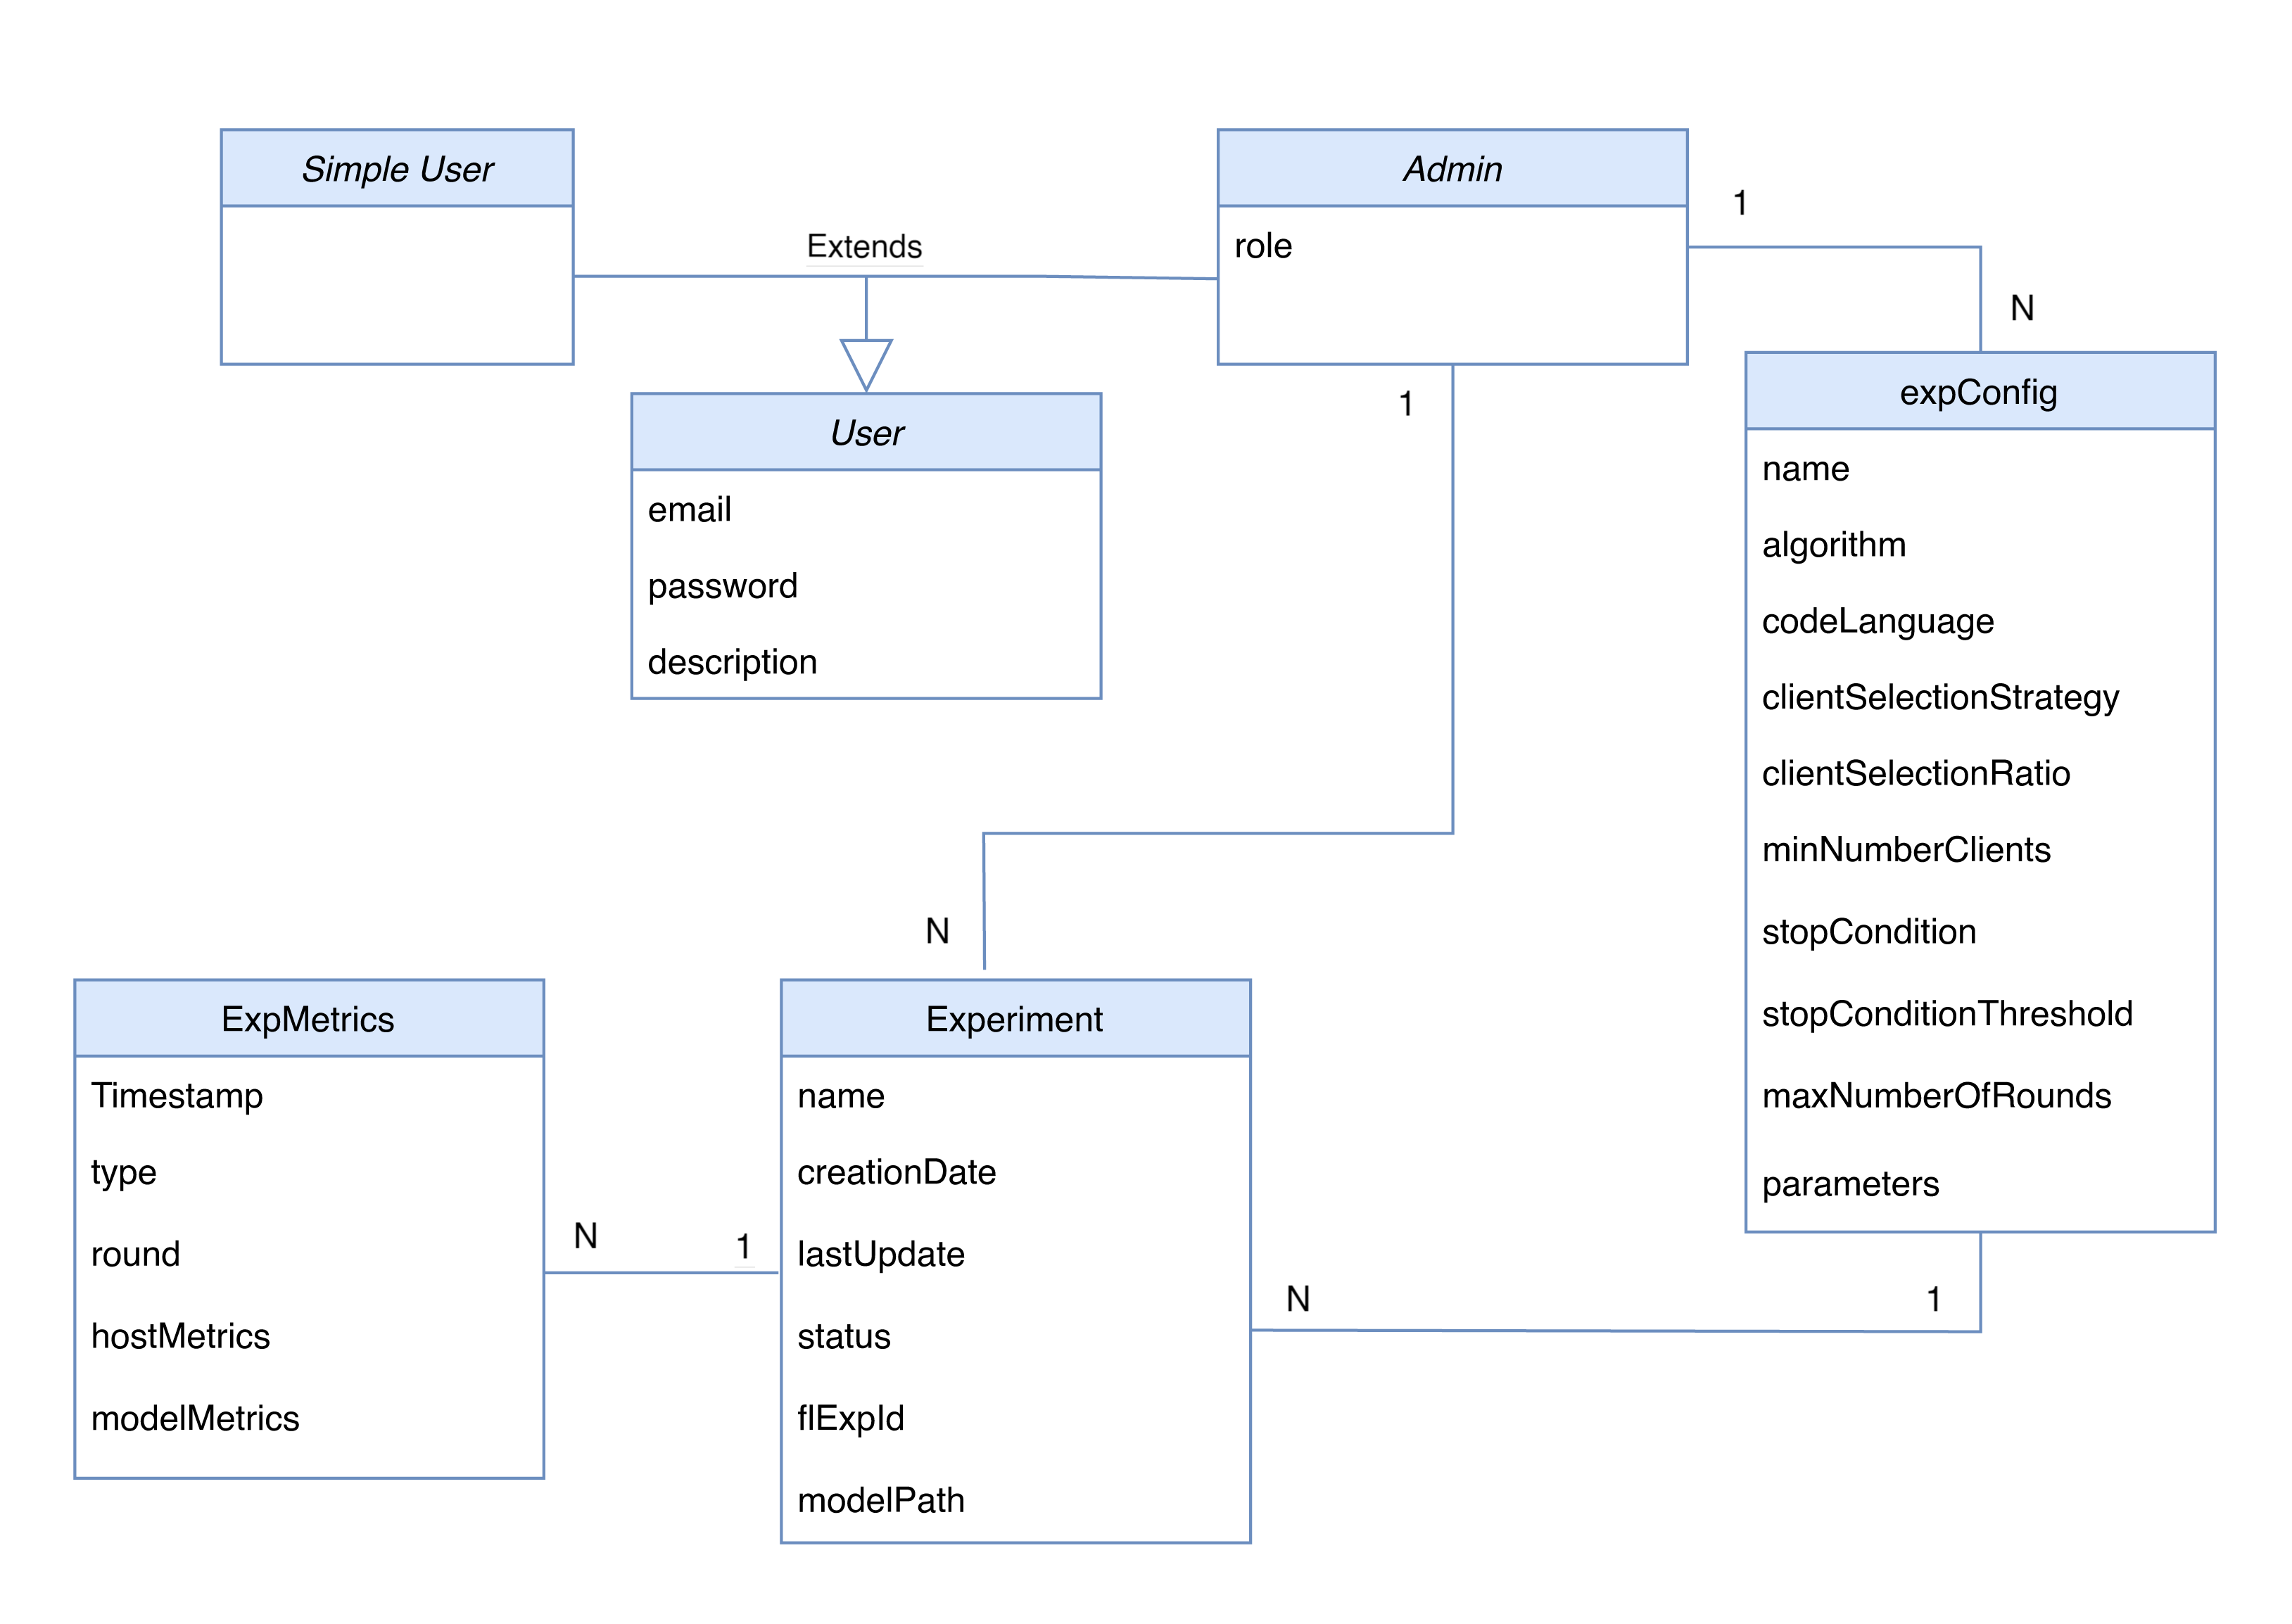
\includegraphics[width=0.8\textwidth]{images/2_analisys/FL_class_diag.png}
    \caption{Class Diagram}
    \label{fig:class_diagram}
\end{figure}

\section{Sequence Diagrams}

The sequence diagrams of the project are presented in this subsection.

